% This document is based on http://math.shinshu-u.ac.jp/~hanaki/beamer/beamer.html
\documentclass[dvipdfmx,cjk]{beamer}
%\documentclass[dvipdfm,cjk]{beamer} % オプションは環境や利用するプログラムによって変える
%\documentclass[dvips,cjk]{beamer}
\usepackage{amsmath}
\usepackage{amssymb}
\usepackage{amsfonts}
\usepackage{latexsym}


% しおり(PDF にしたときの目次)の文字化け防止
\AtBeginDvi{\special{pdf:tounicode 90ms-RKSJ-UCS2}}
%\AtBeginDvi{\special{pdf:tounicode EUC-UCS2}}

% 右下のアイコンを消す
\setbeamertemplate{navigation symbols}{}

% テーマ
\usetheme{CambridgeUS}
%\usetheme{Boadilla}           %% Beamer のディレクトリの中の
%\usetheme{Madrid}             %% beamerthemeCambridgeUS.sty を指定
%\usetheme{Antibes}            %% 色々と試してみるといいだろう
%\usetheme{Montpellier}        %% サンプルが beamer\doc に色々とある。
%\usetheme{Berkeley}
%\usetheme{Goettingen}
%\usetheme{Singapore}
%\usetheme{Szeged}

\usecolortheme{rose}          %% colortheme を選ぶと色使いが変わる
%\usecolortheme{albatross}

%\useoutertheme{shadow}                 %% 箱に影をつける
\usefonttheme{professionalfonts}       %% 数式の文字を通常の LaTeX と同じにする

%\setbeamercovered{transparent}         %% 消えている文字をうっすらと表示する
%\setbeamertemplate{theorems}[numbered]  %% 定理に番号をつける
\newtheorem{thm}{Theorem}[section]
\newtheorem{proposition}[thm]{Proposition}
\theoremstyle{example}
\newtheorem{exam}[thm]{Example}
\newtheorem{remark}[thm]{Remark}
\newtheorem{question}[thm]{Question}
\newtheorem{prob}[thm]{Problem}
\newtheorem{rev}[thm]{Review}
\DeclareMathOperator{\argmin}{argmin}

\AtBeginSection[]{
    \frame{\tableofcontents[currentsection, hideallsubsections]} %目次スライド
}

% メタ情報
\begin{document}
\title[]{数学を「扱う」ことの包摂を考える}
\author[]{理学部 1SC22317Y 照屋 佑喜仁}
\institute[]{}
\date{\today}

% タイトルスライド
\begin{frame}
    \titlepage
\end{frame}

% 目次(\section 名が自動で挿入される)
\begin{frame}
    \tableofcontents
\end{frame}

\section{数学を「扱う」とはどういうことか?}
\begin{frame}
    \frametitle{数学を「扱う」とはどういうことか?}
    数学は理論的で中立な学問\\
    共通語という視点もある

    $\longrightarrow$だが「扱える」のは,誰にとっても平等か?

    \begin{itemize}
        \item 視覚や言語,認知の差が排除を生む可能性
        \item アクセス手段がなければ,思考する前に閉ざされる
    \end{itemize}
\end{frame}

\section{包摂されていない例}
\begin{frame}
    \frametitle{包摂されていない例}
    \begin{itemize}
        \item 視覚障害: 数式やグラフが読めない(画像の式やグラフ)
        \item 読み書きのハンディキャップ(ディスレクシア): 記号の構造が混乱を引き起こす
        \item 言語障壁: 専門語・外国語が思考の妨げに
    \end{itemize}
\end{frame}


\begin{frame}
    \frametitle{具体例}
    視覚障害を持つ学生のケース
    \begin{itemize}
        \item 数式,図が画像$\longrightarrow$スクリーンリーダー非対応
        \item 読み上げ不能,点字変換も困難
        \item 近年はスクリーンリーダー対応された数学コンテンツもあるが限定的
        \item もし読み上げ可能もしくは点字表示可能であったとしても,それが理解に十分に働くか
    \end{itemize}
    \begin{columns}
        \begin{column}{0.5\textwidth}
            \begin{figure}
                \centering
                
\includegraphics[scale=0.1]{expanding.png}
                \caption{視覚障害者向けの数式のオーディオ表現の研究}
            \end{figure}
        \end{column}
        \begin{column}{0.5\textwidth}
            \begin{figure}
                \centering
                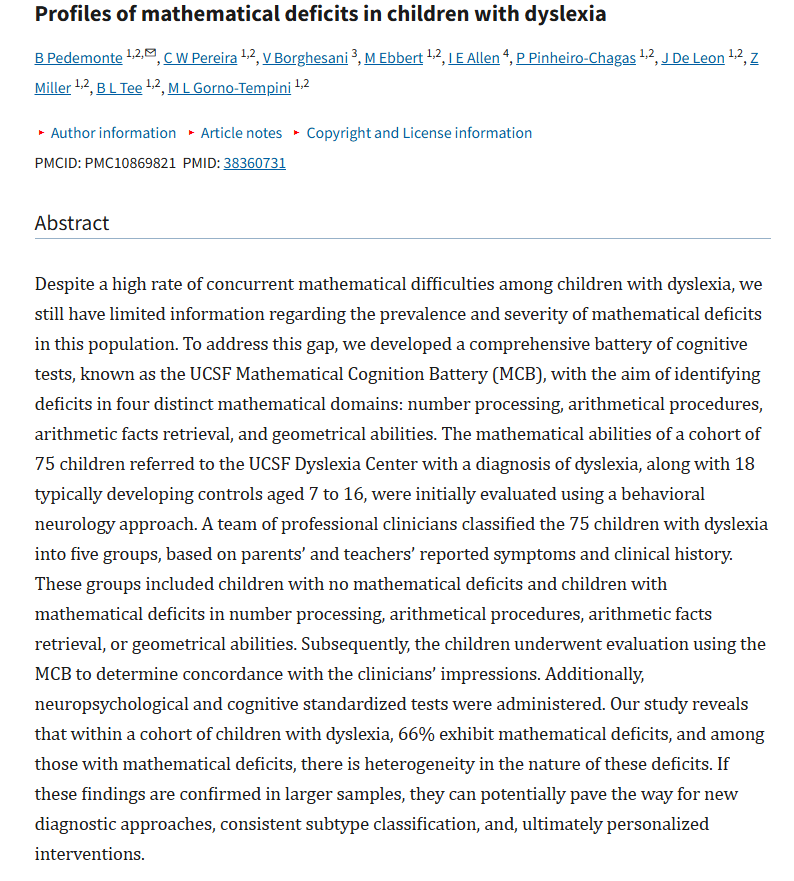
\includegraphics[scale=0.1]{profiles.png}
                \caption{ディスレクシアの数学能力の考察 どのように教育していくかの手がかりになる}
            \end{figure}
        \end{column}
    \end{columns}
\end{frame}

\section{数学を扱う権利とは何か?}
\begin{frame}
    \frametitle{数学を扱う権利とは何か?}
    \begin{itemize}
        \item 数式を読む・操作する権利$=$アクセスの保証
        \item 数学的思考は本来,誰にでも開かれうることが好ましい
        \item 技術,制度,意識からの包摂が必要
    \end{itemize}
\end{frame}

\section{参考文献一覧}
\begin{frame}
    \frametitle{参考文献一覧}
    \begin{itemize}
        \item IES(2011) Expanding Audio Access to Mathematics Expressions by Students with Visual Impairments via MathML
        \item nature(2024) Profiles of mathematical deficits in children with dyslexia
    \end{itemize}
\end{frame}

\end{document}
